\documentclass[10pt, a4paper, onecolumn]{scrartcl}
\usepackage{cite}  
\usepackage{times}
\usepackage{amsmath}
\usepackage{amsfonts}
\usepackage{amssymb}
\usepackage{graphicx}
\usepackage{listings}
\usepackage{enumitem} % used for list - no spaces between items
\usepackage[english]{babel} % English language/hyphenation
\usepackage[top=2cm, bottom= 3.2cm, left=2cm, right=2cm, columnsep=0.6cm]{geometry}
\usepackage{color} %red, green, blue, yellow, cyan, magenta, black, white
\definecolor{mygreen}{RGB}{28,172,0} % color values Red, Green, Blue
\definecolor{mylilas}{RGB}{170,55,241}
\usepackage{fancyhdr}
\pagestyle{fancyplain}
\fancyhead{}
\renewcommand{\headrulewidth}{0pt} % Remove header underlines
\fancyfoot[L]{} % Empty left footer
\fancyfoot[C]{} % Empty center footer
\fancyfoot[R]{\thepage} 
\usepackage{tikz}
\usetikzlibrary{shapes.geometric,arrows}

\usepackage{sectsty} % Allows customizing section commands
\sectionfont{\centering\large\textbf}
\subsectionfont{\flushleft\normalsize\normalfont\textbf}
\subsubsectionfont{\flushleft\normalsize\normalfont\textit}
%\allsectionsfont{\centering} % Make all sections centered

\setlength\parindent{0pt} % remove all indentations in document

%----------------------------------------------------------------------------------------
%	BEGIN DOCUMENT
%----------------------------------------------------------------------------------------
\newcommand{\horrule}[1]{\rule{\linewidth}{#1}}

\begin{document}
	
	\title{\normalfont \normalsize
		\textsc{University of Witwatersrand, Department of Electrical Engineering} \\ [10pt]
		\horrule{0.5pt} \\ [10pt]
		\huge Shopping Route Recommender \\ Sprint Planning Document \\
		\horrule{2pt} \\ [10pt]}
	\author{\textbf{\normalsize{Luka Cakic (671913), Ronen Freeman (386910), Devin Taylor (603956) and Matthew Marsden (609293)}} \\ [10pt]}
	\date {\normalsize \today}
	
	\maketitle
	
	\section{Software Development Life-Cycle Model}
	
		The life-cycle model that the group collectively decided upon are the agile models. The primary motivation for this decision is that changes in project requirements and deliverables during development of such a project in inevitable. In addition, the project is developed based on customer collaboration and not on a contractual negotiation. An agile method was preferred to that of the Waterfall method due to the possibility of the project having rapidly changing requirements based on customer desirables as well as there being tight time constraints suggesting that incrementation development would be preferable over a sequential development process. In addition, as a result of the project requirement potentially changing throughout development, the sequentiality of the Waterfall model cannot be followed, as a result of this model following a method whereby the project requirements are fully defined and known in advance. For these stated reasons the chosen life-cycle model is that of an agile approach. 
		
		\subsection{SCRUM}
		
			In order for Shopping Route Recommender to be a user interactive application, the development team has approached the application's development and aspects as potential users themselves. In effect, this allows "users" to work continuously within the development team, with continuous considerations made towards end user interests. As a result of this, the development process is a team-based approach. The control of conflicting ideas, needs and interests must therefore be adequately managed due to the close collaboration of each development team member. The co-operation amongst the team must be maximised, and communication is vital for successful completion of project tasks. For the reasons stated, the chosen agile process is the SCRUM method. Taking all the aforementioned considerations into account, the SCRUM method ultimately allows a team to maximise productivity.  The fact that there are multiple developers working on the project it is necessary to divide up the work ensuring a faster completion time. In order to do this multiple aspects of this project will be developed in parallel. As a result of this the constant feedback for development sprints, proposed by the SCRUM method, provide additional motivation for the selection of the SCRUM method.
		
	\section{SCRUM Roles}
	
		\subsection{Product Owner}
		
			As there is no direct interfacing with a client in this project there is no need to dedicate a specific group member to being the product owner. As an alternative to this, the team will function collectively as the product owner and will therefore decide as a group what should be placed in the sprint backlog. In addition, the team will collectively negotiate a release date for the product. The feature and priority adjustments will also be collectively decided. 
			
		\subsection{Scrum Master}
		
			The Scrum master for the project will be Devin Taylor. This is primarily due to this members ability to manage time efficiently and to work effectively with a team. He is the most influential group member capable of presenting and inflicting  managerial decisions. As a direct result he also ensures the team is fully functional and that there exists close co-operation across all team roles and functions. He is also capable of representing the management of the project if necessary.  
			
		\subsection{Development Team}
		
			All group members will form part of the group of developers. The main reason for this is due to the limited number of group members available thus the consideration of delivery date is a priority. Therefore, Luka Cakic, Matthew Marsden, Ronen Freeman and Devin Taylor will all form an integral part of the developer team. As Devin Taylor is also the Scrum master, the time dedicated to developing will be less than that of the remaining group members. All the members are cross-functional and demonstrate the necessary skills to complete the web application. Some of the development team's roles include the programming, testing and customer needs analysis of the project. 
	
	\section{SCRUM Planning}
	
		One of the ways in which the group plans on both implementing and monitoring the SCRUM method is through an application called Trello. Trello forms an important backbone to the structure of the SCRUM method planning, by providing a carded system. Each card forms part of a specific sprint, the cards can be taken by individual group members and upon completion of the tasks on the card (in the allocated time frame), the member updates the progress of the task. In doing so, the other group members are informed of all the individual member's project progress. A screen shot of the board currently being used can be seen below. 
		
		\begin{figure}[h!]
			\centering
			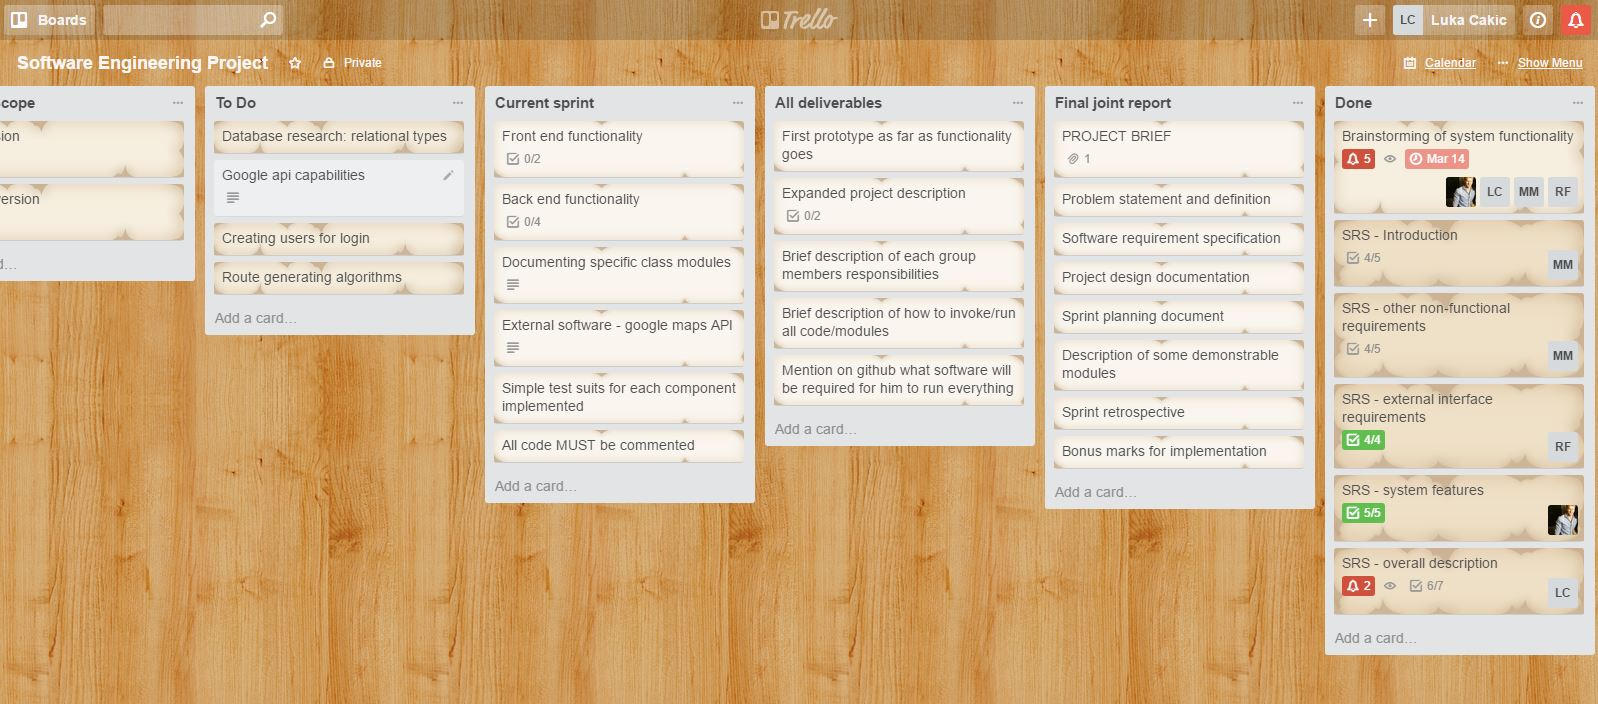
\includegraphics[scale = 0.4]{../images/Trello.JPG}
			\caption{Trello board used for project development}
			\label{menu}
		\end{figure}
		
		\subsection{Project Predecessor Tasks: 18 February}
			
			\begin{itemize}
				\item Create the project backlog for the SCRUM procedure. This involves identifying the customer requirements, the developer team abilities and the list of project priorities that the team need to address during the project sprints. 
				\item The backlog must thereafter be prioritised. 
				\item Set up a sprint planning meeting
					\begin{itemize}
						\item negotiate the duration of the sprints 
						\item select the target backlog for the sprint
						\item clarify sprint requirements
						\item break the sprint requirements into project tasks
					\end{itemize}
			\end{itemize}
		
		\subsection{Sprint 1: 18 February - 26 February}
		
			\begin{itemize}[noitemsep]
				\item The first portion of this sprint is to familiarise the group with Git and the GitHub platform. This involves configuring Git with each group members personal computers 
				\item The next task is to create a project on GitHub
				\item The group is then expected to choose a project topic that will be focused on for the duration of this project
				\item An expanded description of the selected project, distinctly describing the front- and back-ends is to to be provided
				\item The description must also detail the expected inputs and outputs of the system
				\item The responsibilities of each paired group of students must also be detailed in this submission
				\item The documentation of this sprint must be uploaded onto GitHub such that it can be expanded upon at later stages in the development of the project
			\end{itemize}
			
		\subsection{Sprint 2: 3 March - 10 March}
		
			\begin{itemize}[noitemsep]
				\item Set up a sprint planning meeting
					\begin{itemize}
						\item identify the duration of this sprint
						\item select the item targets from the backlog for this sprint
						\item break the sprint requirements into project tasks
					\end{itemize}
				\item The initial stage of this sprint is to firstly select a software development life-cycle (SDLC). The choice must be based on Agile SDLC
				\item The second stage is for the group members to choose a system architecture
				\item The development team must also focus on choosing an appropriate Front End interface method
				\item In order for the system to be fully functional an appropriate Back End must be designed. This involves selecting an HTTP server and an appropriate Database Management System (DBMS)
				\item Supporting API's are also brought forward, discussed and the choices are made clear with regard to the requirements of the system
				\item With all the aforementioned decisions being made, the main purpose of this sprint is to produce the first draft of a detailed Software Requirement Specification				
			\end{itemize}
		
		\subsection{Sprint 3: 24 March - 4 April}
				
			\begin{itemize}[noitemsep]
				\item Set up a sprint planning meeting
					\begin{itemize}
						\item identify the duration of this sprint
						\item select the item targets from the backlog for this sprint
						\item break the sprint requirements into project tasks, identify the components that revolve primarily around the system prototype
					\end{itemize}
				\item Finalise the structure of the back-end and front-end of the prototype. This includes decisions revolving around the frameworks, languages as well as overall appearance of the project
				\item Configure the HTTP server
				\item Configure the database to conform with the structure of the HTTP server
				\item Decide what \texttt{css} styles are applicable to the project
				\item Configure the database to interact with the front-end through the use of an interfacing language
				\item Integrate front-end with back-end
				\item Finalise system prototype
				\item Write test-code to ensure the prototype functions as expected
			
		\subsection{Sprint 4: 5 April - 11 April}
				\item Set up a sprint planning meeting
				\begin{itemize}
					\item identify the duration of this sprint
					\item select the item targets from the backlog for this sprint
					\item break the sprint requirements into project tasks, identify the required documentation for the system
				\end{itemize}
				\item Finalise the project's software requirement specification documentation
				\item Construct the project's software design documentation
				\item A document describing how the final system is invoked must be created
				\item The Front End detailing must be updated and described fully, including describing the respective views accessible by all the web application users
				\item The Back End must also be detailed fully and the techniques describing its configuration and implementation must be finalised
				\item The writing and documentation of some important class modules must be produced, these must identify and illustrate the key aspects of the implemented web application solutions
				\item Reflect on the performance of the SCRUM method for the project
			\end{itemize}	
				
				
				

				
			
			
	
	
\end{document}